\documentclass{article}
\usepackage[utf8]{inputenc}
\usepackage{geometry}
\geometry{
 a4paper,
 total={170mm,257mm},
 left=20mm,
 top=20mm,
}
\usepackage{graphicx}
\usepackage{titling}
\usepackage{listings}
\usepackage[hyphens]{url} 
\usepackage{listings}
\usepackage{xcolor}
\usepackage{graphicx}
\usepackage{subcaption}

\definecolor{codegreen}{rgb}{0,0.6,0}
\definecolor{codegray}{rgb}{0.5,0.5,0.5}
\definecolor{codepurple}{rgb}{0.58,0,0.82}
\definecolor{backcolour}{rgb}{0.95,0.95,0.92}

\lstdefinestyle{mystyle}{
    backgroundcolor=\color{backcolour},   
    commentstyle=\color{codegreen},
    keywordstyle=\color{magenta},
    numberstyle=\tiny\color{codegray},
    stringstyle=\color{codepurple},
    basicstyle=\ttfamily\footnotesize,
    breakatwhitespace=false,         
    breaklines=true,                 
    captionpos=b,                    
    keepspaces=true,                 
    numbers=left,                    
    numbersep=5pt,                  
    showspaces=false,                
    showstringspaces=false,
    showtabs=false,                  
    tabsize=2
}

\lstset{
    language=Python,
    frame=single,
    backgroundcolor=\color{lightgray},
    basicstyle=\ttfamily\footnotesize,
    keywordstyle=\color{blue},
    commentstyle=\color{green!60!black},
    stringstyle=\color{red},
    showstringspaces=false
}

\usepackage{hyperref}
\usepackage{glossaries} % Ajout du package pour le glossaire

\title{Agent intelligent avec Gymnasium}
\author{Mathis A., Ryan C., Samuel M.}
\date{\today}
 
\usepackage{hyperref}
\usepackage{fancyhdr}
\fancypagestyle{plain}{%  the preset of fancyhdr 
    \fancyhf{} % clear all header and footer fields
    \fancyfoot[L]{\thedate}
    \fancyfoot[R]{
\includegraphics[width=2cm]{UQAC_Logo.png}} % Logo et numéro de page en bas à droite
    \fancyhead[L]{Agent intelligent avec Gymnasium}
    \fancyhead[R]{\theauthor}
}

% Appliquer le même style à toutes les pages
\pagestyle{fancy}
    \fancyhead[L]{Agent intelligent avec Gymnasium}
    \fancyhead[R]{\theauthor}
\fancyfoot[L]{\thedate}
\fancyfoot[R]{
\includegraphics[width=2cm]{UQAC_Logo.png}} % Logo et numéro de page en bas à droite

\makeatletter
\def\@maketitle{%
  \newpage
  \null
  \vskip 1em%
  \begin{center}%
  \let \footnote \thanks
    {\LARGE \@title \par}%
    \vskip 1em%
    %{\large \@date}%
  \end{center}%
  \par
  \vskip 1em}
\makeatother

\usepackage{lipsum}  
\usepackage{cmbright}

\begin{document}

\maketitle
\noindent\begin{tabular}{@{}ll}
    Réalisé par :\\
        & Mathis Aulagnier - AULM12040200 \\
        & Ryan Collobert - COLR28120200 \\
        & Samuel Madrigal - MADS23060200 \\
        \\
    Cours :  &  8INF974 – ATELIER PRATIQUE EN INTELLIGENCE ARTIFICIELLE II \\
\end{tabular}

\clearpage

\section{Introduction}

\subsection{L'environnement Gymnasium et ses origines}

\quad Gymnasium représente l'évolution du projet Gym initialement développé par OpenAI. Cette bibliothèque Python offre une interface standardisée pour développer et tester des algorithmes d'apprentissage par renforcement (RL) dans divers environnements. L'objectif principal de Gymnasium est de fournir un cadre uniforme permettant aux chercheurs et développeurs d'implémenter, comparer et partager leurs algorithmes dans des conditions contrôlées.

\subsection{L'héritage Atari en apprentissage par renforcement}

\quad Les jeux Atari occupent une place particulière dans l'histoire de l'apprentissage par renforcement. En 2013, DeepMind a révolutionné le domaine avec DQN (Deep Q-Network), démontrant qu'un agent IA pouvait apprendre à jouer à des jeux Atari directement à partir des pixels de l'écran, sans connaissance préalable des règles. Cette avancée majeure a propulsé le deep reinforcement learning sur le devant de la scène.\\

Les jeux Atari présentent plusieurs avantages comme environnements de test : ils sont suffisamment complexes pour être intéressants mais assez simples pour permettre des expérimentations rapides, tout en offrant une diversité de défis (jeux d'action, de stratégie, de réflexion). C'est pourquoi Gymnasium intègre une collection complète de ces jeux.

\subsection{Les fondements du Reinforcement Learning}

\quad Le Reinforcement Learning (RL) est une partie de l’intelligence artificielle où un agent apprend à prendre des décisions en interagissant avec son environnement. À chaque étape, l'agent : 
\begin{itemize} 
    \item Observe l'état actuel de l'environnement
    \item Choisit une action selon sa politique (policy)
    \item Reçoit une récompense reflétant la qualité de cette action
    \item Observe le nouvel état résultant
\end{itemize}

\quad L'objectif est de maximiser la somme des récompenses futures. Contrairement à l'apprentissage supervisé, le RL ne nécessite pas d'exemples étiquetés, mais apprend par essai-erreur.

\subsection{L'algorithme MCTS et autres approches de RL}

\quad Le Monte Carlo Tree Search (MCTS) est une méthode puissante pour résoudre des problèmes de décision séquentiels, particulièrement efficace dans les jeux à somme nulle comme les échecs ou le go. Le MCTS construit un arbre de recherche asymétrique en privilégiant les branches les plus prometteuses, équilibrant exploration (découverte de nouvelles stratégies) et exploitation (utilisation des connaissances acquises).\\

Au-delà du MCTS, plusieurs familles d'algorithmes coexistent dans le domaine du RL. Ces derniers peuvent être catégorisés  comme "on-policy" (apprennent de leur propre comportement) ou "off-policy" (apprennent d'un comportement différent, souvent plus exploratoire).\\

Ici, nous utiliserons principalement le MCTS qui suit sa politique actuelle et le DQN un algorithme Off-policy qui combine réseaux de neurones et qui recherche la solution optimale. Nous avons également utilisé, durant nos explorations, A2C(on-policy) et Q-Learning(off-policy).

\clearpage

\section{Explorer le Reinforcement Learning avec Blackjack}

\subsection{Premier pas dans l'apprentissage par renforcement}

\quad Pour débuter notre exploration du reinforcement learning avec Gymnasium, nous avons choisi de commencer par un environnement simple mais instructif : le Blackjack. Ce choix s'explique par notre désir d'appréhender les bases du RL sans être immédiatement confrontés aux complexités des interfaces graphiques d'Atari. Le Blackjack fait partie des environnements "Toy Text" de Gymnasium, spécialement conçus pour être élémentaires avec des espaces d'états et d'actions de taille réduite et discrets (2 dans ce cas).\\

Les règles sont légèrement modifiées par rapport au jeu de casino traditionnel. Dans cette version, les options de "doubler la mise" ou de "séparer les paires" ne sont pas disponibles, et le joueur est obligé de tirer en dessous de 12, simplifiant ainsi l'espace des décisions.

\subsection{Implémentation d'un agent Q-learning}

\quad Pour résoudre ce problème, nous avons implémenté un agent utilisant l'algorithme Q-learning, une méthode off-policy qui apprend la valeur optimale de chaque paire état-action. Les principes clés de notre implémentation sont les suivants.\\

Notre agent utilise une stratégie epsilon-greedy pour équilibrer exploration (essai de nouvelles actions) et exploitation (utilisation des connaissances acquises). Au début, l'agent explore beaucoup (epsilon proche de 1), puis progressivement privilégie l'exploitation à mesure que l'apprentissage progresse (epsilon diminue).

\subsection{Évolution de la politique et convergence}

\quad Pour suivre l'évolution de notre agent, nous avons visualisé sa politique toutes les 100 000 itérations. Les visualisations montrent la stratégie de l'agent selon deux dimensions : 
\begin{itemize} 
    \item  La carte visible du croupier (axe des x)
    \item La somme des cartes du joueur (axe des y)
\end{itemize}

    \subsubsection{Phase initiale (premiers épisodes)}
    
    \quad Durant les premiers épisodes, la politique de l'agent était essentiellement aléatoire. Les décisions ne suivaient aucun motif cohérent, témoignant d'un manque d'expérience et de connaissance du jeu.\\
    
    \begin{figure}[ht]
        \centering
        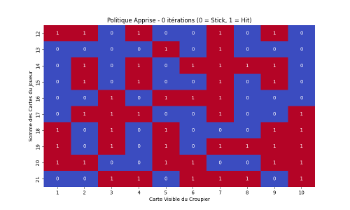
\includegraphics[width=0.8\textwidth]{1.png}
        \caption{image a mettre ici}
    \end{figure}

    \subsubsection{Phase intermédiaire (vers 300 000 épisodes)}
    
    \quad À ce stade, des motifs ont commencé à émerger. L'agent a appris à être plus prudent lorsque sa somme approchait 21 et à prendre plus de risques quand le croupier montrait des cartes à valeur élevée. Cependant, certaines décisions semblaient encore sous-optimales.\\

    \begin{figure}[ht]
        \centering
        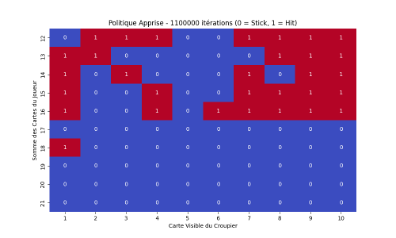
\includegraphics[width=0.8\textwidth]{2.png}
        \caption{image a mettre ici}
    \end{figure}

    \subsubsection{Phase finale}
    
    \quad Après un million d'épisodes, la politique de l'agent a convergé vers une stratégie remarquablement similaire à la stratégie optimale du Blackjack. L'agent a clairement appris à :
    \begin{itemize} 
        \item Rester prudent (stick) avec des sommes élevées (17-21)
        \item Adapter sa stratégie en fonction de la carte visible du croupier, prenant plus de risques quand le croupier a une carte forte (7-10, As)
    \end{itemize}

    \clearpage
    
    \begin{figure}[ht]
        \centering
        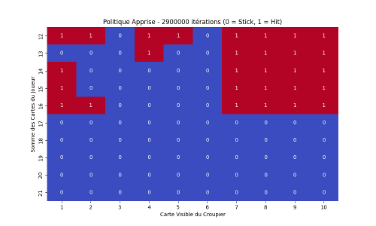
\includegraphics[width=0.8\textwidth]{3.png}
        \caption{image a mettre ici}
    \end{figure}

\subsection{Comparaison avec la stratégie optimale théorique}

\quad La stratégie finale de notre agent correspond parfaitement à la stratégie optimale du Blackjack, compte tenu des règles spécifiques de cet environnement. Notre agent a correctement appris que :
\begin{itemize} 
    \item Il faut être plus conservateur avec des sommes élevées (17+)
    \item Entre 12 et 16, la décision dépend fortement de la carte du croupier
\end{itemize}

\begin{figure}[ht]
    \centering
    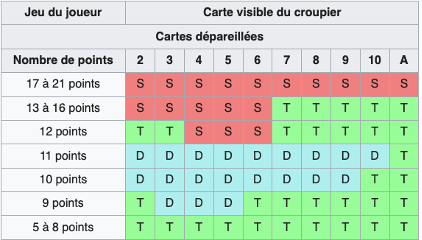
\includegraphics[width=0.7\textwidth]{4.png}
    \caption{image a mettre ici}
\end{figure}

Cette correspondance avec la théorie optimale du Blackjack confirme l’efficacité de notre implémentation du Q-learning et nous a naturellement conduits à tester notre agent sur un jeu plus complexe : le Breakout.

\clearpage

\section{Exploration de l'environnement Breakout avec A2C et Stable-Baselines3}

\subsection{Différences avec le Blackjack}

\quad Contrairement au Blackjack, Breakout présente une complexité accrue avec un espace d'observation visuel et une dynamique temporelle. L'analyse de l'environnement révèle :

\begin{figure}[ht]
    \centering
    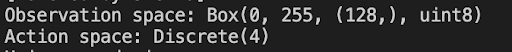
\includegraphics[width=0.8\textwidth]{5.png}
    \caption{image a mettre ici}
\end{figure}

Ces informations nous indiquent que :
\begin{itemize} 
    \item L'agent reçoit des observations sous forme de tableaux d'entiers (0-255) de dimension 128, représentant une version prétraitée de l'image du jeu.
    \item L'agent peut effectuer 4 actions discrètes : ne rien faire, déplacer la raquette à gauche, déplacer la raquette à droite, ou lancer la balle.
\end{itemize}

Nous avons également exploré les différentes options de rendu (render modes) disponibles dans Gymnasium, permettant de visualiser l'environnement de différentes manières : humain (affichage visuel), RGB (capture d'écran brute) ou ASCII (représentation textuelle).

\subsection{Utilisation de Stable-Baselines3}

\quad Pour relever ce défi plus complexe, nous avons adopté Stable-Baselines3, une bibliothèque qui offre des implémentations optimisées d'algorithmes de reinforcement learning. Cette bibliothèque présente plusieurs avantages majeurs :
\begin{itemize} 
    \item Implémentations fiables et testées : Les algorithmes sont implémentés selon les standards académiques et testés rigoureusement.
    \item Interface unifiée : Tous les algorithmes partagent une API commune, facilitant l'expérimentation avec différentes approches.
    \item Intégration transparente avec Gymnasium : La bibliothèque est conçue pour fonctionner nativement avec les environnements Gymnasium.
    \item Compatibilité avec TensorBoard : Permet de suivre et visualiser les métriques d'entraînement en temps réel.
\end{itemize}

Pour notre agent Breakout, nous avons sélectionné l'algorithme A2C, une méthode qui combine les avantages des approches basées sur la valeur et celles basées sur la politique. A2C fonctionne selon les principes suivants :
\begin{itemize} 
    \item Une Architecture Fouble avec un réseau "Actor" (acteur) qui détermine quelle action prendre dans un état donné et un réseau "Critic" (critique) qui évalue la valeur de l'état actuel.
    \item Une Fonction d'Avantage : L'algorithme utilise une fonction d'avantage qui mesure combien une action est meilleure que la moyenne des actions dans un état donné, ce qui réduit la variance lors de l'apprentissage.
\end{itemize}

\subsection{Résultats et analyse des performances}

\quad L'entraînement de notre agent sur l'environnement Breakout a montré une amélioration significative des performances :
\begin{verbatim}
```bash
_____Randomly initialized model_____
Mean reward: 1.5 +/- 0.6708203932499369
____________________________________
_____Trained model_____
Mean reward: 14.8 +/- 5.114684741017769
____________________________________
```
\end{verbatim}

\clearpage

\begin{figure}[ht]
    \centering
    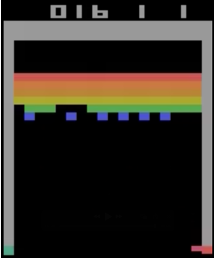
\includegraphics[width=0.3\textwidth]{6.png}
    \caption{image a mettre ici}
\end{figure}

Ces résultats démontrent que notre agent a appris à jouer au jeu de manière efficace, multipliant par presque 10 le score obtenu par un agent à politique aléatoire.

    \subsubsection{Analyse des métriques TensorBoard}
    
    \quad TensorBoard nous a permis de visualiser plusieurs métriques clés pendant l'entraînement, offrant des insights précieux sur le processus d'apprentissage.\\

        Métriques de performance de l'agent
        
        \begin{itemize} 
            \item \begin{verbatim}ep_len_mean :\end{verbatim}La durée moyenne des épisodes est passée d'environ 250 à près de 800 pas de temps, indiquant que l'agent survit plus longtemps.
            \item \begin{verbatim}ep_rew_mean :\end{verbatim}La récompense moyenne par épisode a progressivement augmenté pour atteindre environ 21.5, démontrant une amélioration constante de la stratégie.
        \end{itemize}
        
        \begin{figure}[ht]
            \centering
            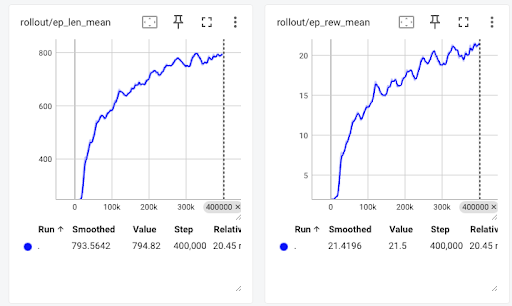
\includegraphics[width=0.8\textwidth]{7.png}
            \caption{image a mettre ici}
        \end{figure}
    
        Métriques d'apprentissage
        
        \begin{itemize} 
            \item \begin{verbatim}entropy_loss :\end{verbatim}La perte d'entropie a diminué (s’est rapprochée de 0), indiquant que la politique devient plus déterministe au fil du temps, à mesure que l'agent découvre les actions optimales.
            \item \begin{verbatim}explained_variance :\end{verbatim}Cette métrique oscille autour de 0.75, ce qui est un bon indicateur que le critique prédit raisonnablement bien les retours attendus.
            \item \begin{verbatim}learning_rate :\end{verbatim}Indique le taux d’apprentissage utilisé pour ce modèle à 0.0007. Il est constant dans cet algorithme.
            \item \begin{verbatim}policy_loss :\end{verbatim}La perte de politique reste faible et stable, signe que l'apprentissage de l'acteur progresse de manière équilibrée.
            \item \begin{verbatim}value_loss :\end{verbatim}Cette perte oscille fortement alors qu’elle devrait diminuer progressivement, montrant que le critique s'améliore dans ses prédictions.
        \end{itemize}
        
        \begin{figure}[ht]
            \centering
            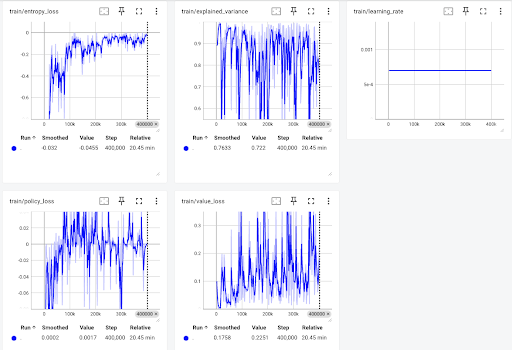
\includegraphics[width=0.8\textwidth]{8.png}
            \caption{image a mettre ici}
        \end{figure}
    
        Globalement, ces métriques révèlent un processus d'apprentissage sain, avec une convergence progressive vers une politique efficace. La stabilité des courbes dans les dernières phases de l'entraînement suggère que notre modèle  n’a pas atteint une performance proche de son potentiel optimal pour la durée d'entraînement allouée.\\
    
        Cette expérience constitue une base solide pour aborder des défis encore plus complexes, notamment la mise en œuvre d'algorithmes comme MCTS pour des jeux à information parfaite comme le Tic-tac-toe et les échecs.

\clearpage

\section{MCTS sur TicTacToe3D : Défis et Limitations}

\subsection{Structure de notre programme}

\quad Nous avons choisi de développer un algorithme de recherche Monte Carlo Tree Search (MCTS) pour le jeu TicTacToe3D, proposé par Gymnasium. Ce choix s'explique par la simplicité du jeu et la rapidité des parties, ce qui facilite l'observation du comportement du MCTS. À l'inverse, un jeu comme les échecs exigerait non seulement un temps de calcul plus important, mais aussi une expertise approfondie pour évaluer la pertinence des décisions prises par l'algorithme.\\

Le TicTacToe3D se joue sur un cube de dimensions 4×4×4, où chaque joueur doit aligner quatre symboles identiques (X ou O) pour l'emporter. La partie s'achève lorsqu'un joueur atteint cet objectif ou lorsque l'ensemble du cube est rempli.\\

Notre programme se structure en trois parties principales :
\begin{itemize} 
    \item Les nœuds, qui permettent d'initialiser un état du jeu, de vérifier s'il a été entièrement exploré et d'identifier son meilleur successeur.
    \item L'algorithme MCTS, qui constitue le cœur de notre implémentation.
    \item Le jeu, où l'on applique le MCTS avec une visualisation des coups joués.
\end{itemize}

\quad L'essentiel du travail s'est naturellement concentré sur le développement et l'optimisation du MCTS, puisqu'il s'agit du moteur décisionnel de notre projet.

\begin{figure}[ht]
    \centering
    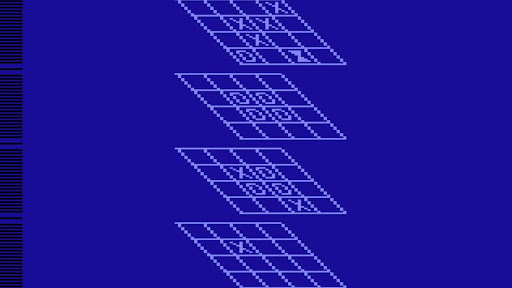
\includegraphics[width=0.7\textwidth]{9.png}
    \caption{Partie de TicTacToe3D}
\end{figure}

\subsection{Implémentations du MCTS}

\quad Face aux défis rencontrés lors du développement, nous avons implémenté l’algorithme MCTS selon deux approches distinctes. Dans les deux cas, nos implémentations assurent la sélection du meilleur enfant dans l’arbre, la gestion des récompenses en fonction des résultats des parties simulées, ainsi que la rétropropagation de ces récompenses vers les nœuds parents.\\

La gestion des récompenses repose sur la fonction “env.step(action)”, qui met à jour l'état du jeu après chaque action. De plus, nous augmentons manuellement la récompense totale lorsqu’une partie atteint un état "terminated", c’est-à-dire lorsqu’un joueur gagne ou que la grille est complètement remplie. La rétropropagation des récompenses est gérée de manière récursive, garantissant ainsi une transmission efficace des informations à travers l’arbre.\\

L’élément central du MCTS est l’expansion de l’arbre. Celui-ci continue de croître tant que tous ses nœuds ne sont pas totalement explorés. Lorsqu’un nœud dispose encore d’actions non exploitées, il sélectionne aléatoirement un coup parmi la liste des actions légales non jouées, puis ajoute un nouveau nœud enfant à l’arbre.\\

L’ensemble de ce processus est orchestré par une fonction de recherche, qui prend en entrée une copie de l’état actuel du jeu et effectue un nombre défini d’itérations pour évaluer les différentes possibilités. Cette itération permet ensuite de déterminer le meilleur coup à jouer dans la partie réelle.

\subsection{Problèmes rencontrés et limites atteintes}

\quad Le premier problème que nous avons rencontré concernait le comportement aléatoire de notre programme. Celui-ci tentait parfois de jouer des coups illégaux, par exemple en plaçant un symbole dans une case déjà occupée, voire en exécutant des actions totalement étrangères au jeu. Pour y remédier, nous avons mis en place une gestion stricte des coups légaux, garantissant que seuls les coups jouables dans des cases vides du TicTacToe3D soient autorisés.\\

Un second problème majeur résidait dans la phase d’exploration du MCTS. Initialement, cette exploration s’effectuait directement dans la partie en cours, rendant le processus totalement aléatoire et dépourvu d’apprentissage réel. Pour y remédier, nous avons adopté une approche différente : au lieu d’explorer l’environnement de jeu réel, nous avons introduit un système de copies permettant d’exécuter les simulations indépendamment, afin d’identifier et de sélectionner uniquement les meilleurs coups.\\

Comme mentionné précédemment, nous avons développé deux versions distinctes du MCTS, chacune présentant ses propres avantages et inconvénients.

    \subsubsection{Problèmes de la première implémentation}
    
    \quad Le premier défaut majeur de cette version est que l'affichage du jeu ne fonctionne pas. Néanmoins, nous avons pu vérifier que le MCTS explore bien et joue des coups en plaçant des “print(informations importantes…)” stratégiques pour suivre l'exécution du programme dans le terminal.\\
    
    Un autre problème notable est que l’exploration suit systématiquement le même schéma, suggérant une mauvaise implémentation de la phase d’expansion du MCTS. De plus, les parties semblent ne jamais se terminer. L’absence d’interface visuelle nous empêche d’identifier clairement la cause de ce comportement. L'action sélectionnée étant représentée par un entier (ex : "l’action choisie est 3"), nous savons seulement que le programme exécute une action légale, sans pouvoir comprendre précisément ce qu’elle implique.

    \subsubsection{Seconde implémentation : améliorations et nouvelles difficultés}
    
    \quad Pour remédier à ces problèmes, nous avons développé une deuxième version du MCTS. Dans cette version, l’affichage fonctionne correctement, aussi bien pour la partie réelle que pour les parties simulées. Cette amélioration nous permet de visualiser le déroulement du jeu, de mieux comprendre les décisions prises par l’algorithme et de vérifier si l’exploration suit un schéma cohérent. Nous avons d’ailleurs constaté que, cette fois, l’exploration n’adopte plus un motif fixe, ce qui est une amélioration.\\
    
    Cependant, cette version introduit un nouveau problème critique : les parties ne se terminent jamais, mais pour une raison différente. L’algorithme choisit systématiquement l’action "0", qui est une action neutre. En analysant le problème, nous avons découvert que la valeur de récompense reste constamment bloquée à 0. Quelle que soit la méthode employée, que ce soit via env.step(action) ou une incrémentation manuelle, la récompense n’évolue pas.\\

    Malgré cela, le programme sélectionne bien un nœud, puisque l’action par défaut est NONE. Le problème ne vient donc pas de l’assignation de l’action au jeu réel, mais de la façon dont nous évaluons et sélectionnons un nœud en fonction de sa valeur, mais la valeur reste toujours bloquée comme indiqué précédemment. Ce problème d'inaction est d’ailleurs similaire à celui que nous avons rencontré lors du développement du MCTS pour les échecs, que nous aborderons dans la section suivante. Toutefois, la solution que nous avons trouvée pour les échecs n’est pas applicable au TicTacToe3D...

\clearpage

\section{MCTS sur Chess : Défis et Limitations}

\subsection{Les défis de l'environnement Chess dans Gymnasium}

\quad Notre exploration du Monte Carlo Tree Search (MCTS) s'est finalement tournée vers les échecs, un défi considérable en matière de complexité computationnelle. Cependant, notre première tentative avec l'environnement "Video Chess" de Gymnasium s'est heurtée à des obstacles majeurs.\\

Le problème fondamental de cet environnement réside dans sa conception basée sur l'émulation Atari, qui reproduit fidèlement l'expérience utilisateur d'un jeu vidéo d'échecs plutôt que de proposer une interface adaptée à l'apprentissage par renforcement. Concrètement, les actions disponibles pour l'agent sont limitées à :
\begin{itemize} 
    \item Ne rien faire
    \item Déplacer le curseur dans quatre directions (haut, bas, gauche, droite)
    \item Sélectionner une case
\end{itemize}

Cette interface présente deux inconvénients critiques pour le MCTS :
\begin{itemize} 
    \item Inefficacité des actions : La grande majorité des séquences d'actions ne produisent aucun changement valide dans l'état du jeu. L'agent doit d'abord sélectionner l'une de ses pièces (10/64 cases au début), puis naviguer correctement pour choisir une case de destination légale (environ 2/64 cases), ce qui représente une probabilité infime de succès par exploration aléatoire.
    \item Absence de connaissance des règles : L'agent n'a aucune notion préalable des règles des échecs, ce qui rend presque impossible la découverte de mouvements légaux par simple exploration.
\end{itemize}

Ces limitations font que l'espace d'actions effectif est extrêmement dilué, rendant la convergence de l'algorithme MCTS pratiquement inatteignable dans un temps raisonnable.

\subsection{Migration vers Chess-py}

\quad Face à ces difficultés, nous avons décidé d'adopter une approche plus adaptée en utilisant la bibliothèque Chess-py. Contrairement à l'environnement Gymnasium, cette bibliothèque offre une interface beaucoup plus appropriée pour l'apprentissage par renforcement appliqué aux échecs, notamment grâce à la fonction `legal\_moves` qui renvoie directement la liste des coups légaux dans une position donnée.\\

Cette fonctionnalité est cruciale pour le MCTS, car elle permet de restreindre drastiquement l'espace d'exploration aux seuls coups valides, éliminant ainsi le problème de dilution des actions rencontré précédemment.\\

Malgré cette amélioration significative de l'interface, notre agent d'échecs basé sur MCTS a continué à présenter des performances très faibles. Un examen approfondi de son comportement a révélé plusieurs problèmes :
\begin{itemize} 
    \item Manque de discernement tactique : L'agent ne semblait pas reconnaître l'intérêt de capturer des pièces adverses. Ce comportement s'explique par le fait que notre implémentation initiale du MCTS ne considérait que les résultats finaux (victoire, défaite ou nulle) sans évaluation intermédiaire des positions.
    \item Arbre d'exploration extrêmement clairsemé** : L'espace des états des échecs est astronomiquement vaste (environ 10\^{}123 parties raisonnables et plus de 10\^{}6000 parties théoriquement possibles). Dans un tel espace, l'exploration aléatoire a une probabilité infime de découvrir des séquences de coups tactiquement pertinentes.
\end{itemize}

Pour remédier au premier problème, nous avons tenté d'intégrer une heuristique simple d'évaluation matérielle dans notre processus de sélection de coups :
\begin{itemize} 
    \item Pion : 1 point
    \item Cavalier/Fou : 3 points
    \item Tour : 5 points
    \item Dame : 9 points
    \item Roi sans valeur car fin de partie
\end{itemize}

L'idée était de guider l'exploration vers des positions où l'agent dispose d'un avantage matériel. Cependant, cette approche n'a apporté qu'une amélioration marginale, rendant l'agent légèrement plus agressif mais toujours fondamentalement mauvais.\\

    \subsubsection{Intégration avec Stockfish : une approche hybride}

    \quad Face à ces limitations, nous avons exploré une approche plus innovante en intégrant Stockfish, un des moteurs d'échecs les plus puissants, comme composant de notre simulation MCTS. Le principe était le suivant :
    \begin{itemize} 
        \item Notre agent choisit un coup initial (selon la politique MCTS)
        \item Stockfish répond avec un coup optimisé (limité à une profondeur de 5 pour maintenir un niveau raisonnable)
        \item L'exploration MCTS continue à partir de cette nouvelle position
    \end{itemize}
    
    Cette approche visait à remplacer la simulation aléatoire traditionnelle du MCTS par une simulation plus "réaliste", guidée par un adversaire compétent. Théoriquement, cela devait permettre d'explorer des lignes de jeu plus pertinentes et d'accélérer l'apprentissage. En effet, lors de coups hasardeux joués par l’ordinateur, stockfish devrait rapidement prendre l’avantage et remporter la partie, laissant place à une nouvelle exploration.\\

    \subsubsection{Limites de l'approche hybride}

    \quad Bien que conceptuellement prometteuse, cette approche hybride s'est heurtée à deux obstacles majeurs :
    \begin{itemize} 
        \item Performance computationnelle : La communication avec Stockfish et le temps de calcul nécessaire à ses analyses rendaient chaque itération du MCTS extrêmement lente, réduisant drastiquement le nombre d'itérations possibles dans un temps donné.
        \item Biais d'apprentissage : Face à un adversaire aussi fort que Stockfish, même limité en profondeur, la grande majorité des explorations se soldaient par des défaites pour notre agent. Cette homogénéité des résultats rendait difficile la différenciation entre les "moins mauvais" coups, tous menant ultimement à la défaite.
    \end{itemize}
    
    L'examen de l'arbre d'exploration confirmait cette tendance : presque toutes les branches explorées se terminaient par une défaite, ce qui empêchait l'algorithme de déterminer une direction préférentielle, tous les coups ayant approximativement la même valeur attendue (négative).\\

    \subsubsection{Réflexions sur les limites du MCTS pur pour les échecs}

    \quad Cette expérience nous a permis de constater les limites fondamentales du MCTS "pur" pour un domaine aussi complexe que les échecs :
    \begin{itemize} 
        \item Complexité combinatoire : L'espace d'états des échecs est tellement vaste qu'une exploration efficace nécessite une forme de connaissance ou d'heuristique préalable pour guider la recherche.
        \item Horizon d'évaluation : Aux échecs, les conséquences d'un coup peuvent ne se manifester que bien plus tard dans la partie. Le MCTS, particulièrement avec des simulations aléatoires, a du mal à capturer ces relations à long terme.
        \item Nécessité d'évaluations intermédiaires : Contrairement à des jeux comme Go où le MCTS a excellé, les échecs bénéficient grandement d'évaluations positionnelles précises à chaque étape, plutôt que de s'appuyer uniquement sur le résultat final.
    \end{itemize}

    Ces observations expliquent pourquoi les moteurs d'échecs modernes les plus performants, comme Stockfish lui-même, s'appuient principalement sur des recherches alpha-beta très profondes enrichies par des évaluations de position sophistiquées, plutôt que sur le MCTS pur. Même AlphaZero, qui utilise une variante de MCTS, intègre un réseau neuronal profond pour l'évaluation des positions et la suggestion de coups, s'éloignant considérablement du MCTS classique.\\

\clearpage

\section{Deep Q-learning (DQN) : Défis et Limitations}

\subsection{Introduction au Deep Q-Learning (DQN)}

\quad Le Deep Q-Learning (DQN) est une méthode de renforcement learning qui combine les réseaux de neurones profonds avec l'algorithme Q-Learning. Il permet à un agent d'apprendre à prendre des décisions optimales dans un environnement donné en maximisant une récompense cumulative. Cette approche est particulièrement efficace pour des environnements complexes, tels que les jeux vidéo dans notre cas, où l'espace d'états et d'actions est vaste et difficile à modéliser manuellement.\\

Cependant, l'application du DQN à des jeux comme les échecs ou les dames présente des défis spécifiques, notamment en raison de la complexité des règles, de la grande taille de l'espace d'états, et de la nécessité de gérer des actions discrètes et continues.

\subsection{Les défis de l'environnement Chess et Checkers dans Gymnasium}

\quad Nous avons initialement choisi d'implémenter notre modèle DQN en utilisant Gymnasium, une bibliothèque populaire pour les environnements de renforcement learning, en raison de sa compatibilité avec des frameworks comme Stable-Baselines3. Cependant, nous avons rapidement rencontré des difficultés liées à la nature des environnements Chess et Checkers.

    \subsubsection{Similarités entre Chess et Checkers}

    \quad Les environnements Chess et Checkers partagent des caractéristiques communes, notamment un espace d'états basé sur un plateau de jeu et des actions discrètes représentant les mouvements possibles des pièces. Pour traiter les images renvoyées par Gymnasium (représentant l'état du plateau), nous avons opté pour l'utilisation d'un réseau de neurones convolutif (CNN) dans notre DQN. Les CNN sont particulièrement adaptés pour extraire des caractéristiques spatiales à partir de données visuelles, ce qui les rend idéaux pour traiter les états du jeu sous forme d'images.

    \subsubsection{Problèmes spécifiques à Gymnasium}

    \quad Malgré ces avantages, nous avons rencontré plusieurs difficultés avec Gymnasium. Par exemple, certaines actions générées par le modèle ne correspondaient pas à des coups valides selon les règles du jeu, ce qui a provoqué des erreurs lors de l'exécution. De plus, la gestion des environnements Chess et Checkers dans Gymnasium s'est révélée moins fiable que prévu, en raison de limitations dans l'implémentation des règles et des récompenses. Par exemple, les déplacements du pointeur ne génèrent aucun point, et les images clignotantes changent sans aucune action de l'agent, ce qui complique l'apprentissage.

\subsection{Les défis de l'environnement Chess-py}
\quad Pour contourner ces problèmes, nous avons décidé de basculer une nouvelle fois vers l'environnement Chess-py, une bibliothèque spécialisée pour les échecs en Python. Contrairement à Gymnasium, Chess-py offre une implémentation plus fiable des règles du jeu et permet une meilleure gestion des coups légaux. Cependant, cette transition a introduit de nouveaux défis.

    \subsubsection{Intégration avec Stable-Baselines3}

    \quad Stable-Baselines3 comme présenté précédemment est conçu pour fonctionner avec des environnements compatibles avec l'API de Gymnasium. Or, Chess-py n'implémente pas nativement cette API. Pour résoudre ce problème, nous avons créé un environnement personnalisé (ChessEnv) dans un fichier à part qui implémente les méthodes standard de Gymnasium, telles que reset(), step(), et render(). Cela nous a permis d'intégrer Chess-py avec Stable-Baselines3 tout en conservant les fonctionnalités nécessaires pour l'entraînement du DQN.

    \subsubsection{Choix du modèle : MLP vs CNN}

    \quad Contrairement aux jeux Atari, où les états sont représentés sous forme d'images, Chess-py fournit une représentation unidimensionnelle du plateau de jeu. Par conséquent, nous avons opté pour un Multi-Layer Perceptron (MLP) plutôt qu'un CNN. Le MLP est plus adapté pour traiter des données structurées et de faible dimension, ce qui correspond à la représentation du plateau dans Chess-py. Ce choix a permis de simplifier l'architecture du modèle tout en maintenant des performances satisfaisantes.

    \subsubsection{Problème avec les coups légaux}

    \quad Un défi majeur rencontré lors de l'utilisation de Chess-py réside dans la gestion des coups légaux. Bien que la fonction legal\_moves permette de restreindre les actions aux coups valides, elle introduit une limitation significative : le nombre de coups légaux disponibles varie considérablement en fonction de la position du jeu, passant d'une trentaine de coups possibles à certains moments à un nombre bien moindre dans d'autres situations.\\

    Cependant, pour que l'agent puisse s'entraîner efficacement avec Stable-Baselines3, l'espace d'actions (self.action\_space) doit être de taille constante. Nous avons donc dû définir un espace d'actions fixe, correspondant à l'ensemble des 4032 coups théoriques (8×8×((8x8)-1)), bien que seule une fraction de ces coups soit réellement jouable à chaque étape. Cette contrainte ralentit considérablement l'apprentissage, car l'agent passe beaucoup de temps à essayer des coups invalides, ce qui entraîne des pénalités et retarde la découverte des stratégies optimales. Avec un nombre limité d'étapes d'entraînement (total\_timesteps=1000000), l'agent commence seulement à comprendre qu'il est pénalisé pour ces tentatives infructueuses, ce qui limite ses performances globales. Cette problématique souligne la nécessité d'une approche plus adaptative pour gérer les coups légaux dans des environnements aussi dynamiques que les échecs.\\
    
    Afin d'avoir un entraînement réalisable dans une période de temps convenable (total\_timesteps=1000000), nous devons donc réduire la plage de possibilité d’actions.


\subsection{Analyse des métriques TensorBoard}

\quad Pour évaluer les performances de notre modèle, nous avons utilisé TensorBoard pour visualiser les métriques d'entraînement, telles que la récompense moyenne par épisode, la perte du réseau, et le taux d'exploration. Ces métriques nous ont permis de suivre la progression de l'apprentissage et d'ajuster les hyperparamètres du modèle en conséquence.

    \subsubsection{Configuration du modèle}

    \quad Nous avons configuré notre DQN avec les hyperparamètres suivants :
    \begin{itemize} 
        \item Taux d'apprentissage (learning rate) : 1e-4 pour les jeux Atari et 1e-5 pour Chess-py, afin de stabiliser l'entraînement.
        \item Taille du replay buffer : 40 000 pour les jeux Atari et 200 000 pour Chess-py, pour permettre une exploration plus approfondie.
        \item Taille du batch : 32 pour les jeux Atari et 64 pour Chess-py, afin d'améliorer la convergence du modèle.
        \item Exploration : Nous avons utilisé un taux d'exploration initial de 1.0, qui diminue progressivement jusqu'à 0.01 pour favoriser l'exploitation des connaissances acquises.
    \end{itemize}

    \subsubsection{Analyse des métriques TensorBoard (en cours d'entraînement)}

    \quad TensorBoard nous a permis de visualiser plusieurs métriques clés pendant l'entraînement, offrant des informations précieuses sur le processus d'apprentissage.\\

    Métriques de performance de l'agent :
    \begin{itemize} 
        \item \begin{verbatim}ep_len_mean :\end{verbatim}La durée moyenne des épisodes est passée d'environ 830 à près de 30 pas de temps, indiquant que l'agent termine les parties de plus en plus rapidement.
        \item \begin{verbatim}ep_rew_mean :\end{verbatim}La récompense moyenne par épisode a augmenté de manière presque exponentielle au début, passant d'environ -550 pour atteindre finalement environ 10, démontrant une nette amélioration de la stratégie. Nous pouvons également observer une phase d'exploration lors d'un changement de stratégie entre les 500 000 et 800 000 pas de temps.
    \end{itemize}

    \begin{figure}[ht]
        \centering
        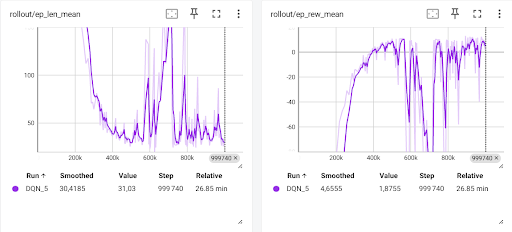
\includegraphics[width=0.8\textwidth]{10.png}
        \caption{image a mettre ici}
    \end{figure}
    
    Métriques d'apprentissage :
    \begin{itemize} 
        \item \begin{verbatim}exploration_rate :\end{verbatim}Le taux d'exploration initial est bien de 1.0, puis diminue progressivement jusqu'à 0.01 à 500 000 pas de temps pour favoriser l'exploitation des connaissances acquises.
        \item \begin{verbatim}learning_rate :\end{verbatim}Le taux d'apprentissage utilisé pour ce modèle est de 10\^{}-5. Il reste constant tout au long de l'entraînement.
        \item \begin{verbatim}loss :\end{verbatim}La perte oscille fortement alors qu'elle devrait diminuer progressivement, montrant que le critique s'améliore dans ses prédictions.
    \end{itemize}

    \begin{figure}[ht]
        \centering
        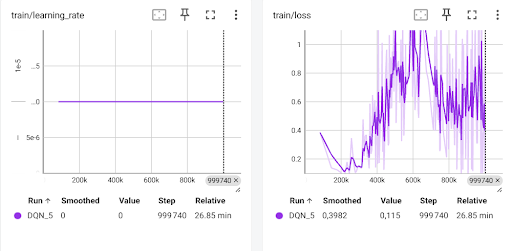
\includegraphics[width=0.8\textwidth]{11.png}
        \caption{image a mettre ici}
    \end{figure}

    \clearpage
    
    \begin{figure}[ht]
        \centering
        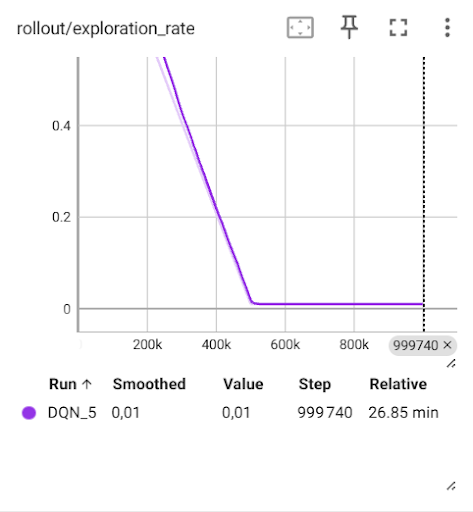
\includegraphics[width=0.5\textwidth]{12.png}
        \caption{image a mettre ici}
    \end{figure}

    Interprétation des résultats :\\

    Globalement, ces métriques révèlent un processus d'apprentissage orienté vers des parties expéditives avec des échecs et mats très agressifs ou des matchs nuls par répétition du même coup trois fois de suite. Cela permet de réduire au maximum les chances d'obtenir des pénalités en jouant un coup interdit (un phénomène qui peut être dû à une sanction trop forte). Cependant, nous pouvons aussi observer que l'agent apprend bien les coups qui ne lui apportent pas de pénalités, mais il semble privilégier ceux qui mènent rapidement à une fin de partie.

\clearpage

\section{Entraînement d'un Agent Ms. Pac-Man avec DQN}

\quad Nous avons développé un agent capable de jouer à Ms. Pac-Man en utilisant un Deep Q-Network (DQN). Contrairement à l’approche MCTS utilisée pour les échecs, l’agent apprend ici à partir de zéro, uniquement par interaction avec l’environnement.\\

L’architecture de l’agent repose sur un réseau de neurones convolutif (CNN). Ce type de réseau est particulièrement adapté au traitement des images, car il permet d’extraire automatiquement des caractéristiques pertinentes. Les CNN capturent des motifs simples comme les murs ou les points, mais aussi des configurations plus complexes comme les positions relatives des fantômes.\\

Pour permettre une meilleure perception temporelle, nous avons intégré une technique de frame stacking. Cette méthode consiste à empiler les quatre dernières images observées, ce qui permet à l’agent de percevoir le mouvement des fantômes et d’anticiper leur trajectoire. Cette approche améliore la prise de décision dans un environnement dynamique.\\

L’algorithme DQN utilisé intègre plusieurs améliorations. L’agent s’entraîne à partir d’un buffer de replay de 100 000 transitions, ce qui permet de briser la corrélation temporelle entre les échantillons. Un réseau cibleest mis à jour toutes les 1000 étapes pour stabiliser l’apprentissage. Le taux d’exploration décroît progressivement de 1.0 à 0.01, permettant à l’agent de passer d’une phase d’exploration à une phase d’exploitation des stratégies acquises. L’apprentissage commence après 10 000 interactions pour garantir une base suffisante de données. L’agent met à jour son réseau toutes les quatre interactions, assurant une régularité dans l’entraînement.\\

Après un million de pas d’entraînement, l’agent a montré une progression constante. La durée moyenne des épisodes a atteint environ 1250 étapes, indiquant une meilleure capacité à survivre plus longtemps dans le labyrinthe. La récompense moyenne par épisode a augmenté jusqu’à environ 1850 points, signe que l’agent a appris à collecter plus efficacement les points tout en évitant les fantômes. Le taux d’exploration a suivi la courbe attendue, passant de 1.0 à 0.01 au fil de l’entraînement.\\

\begin{figure}[ht]
    \centering
    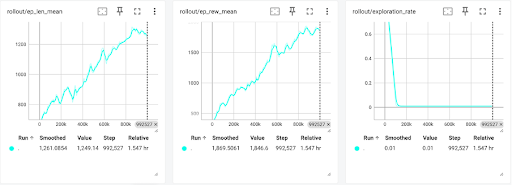
\includegraphics[width=0.9\textwidth]{13.png}
    \caption{image a mettre ici}
\end{figure}

L’agent a développé plusieurs comportements intéressants. Il navigue efficacement dans le labyrinthe, évitant les impasses et optimisant son chemin vers les points. Il anticipe les mouvements des fantômes et ajuste sa trajectoire pour éviter les collisions. Il adopte une stratégie opportuniste en capturant les power-ups et en poursuivant les fantômes vulnérables.\\

Après un million de parties d’entraînement, l’agent atteint un score de 1850 se rapprochant du score moyen d’environ 2400. Il se rapprochant ainsi des performances humaines. Cette progression témoigne de sa capacité à comprendre la dynamique du jeu et à adopter des stratégies efficaces. Un entraînement plus long lui aurait probablement permis d’affiner ses décisions et d’améliorer sa gestion des situations complexes, consolidant ainsi encore davantage sa maîtrise du jeu.

\clearpage

\section{Conclusion}
\quad Ce projet d'apprentissage par renforcement nous a permis d'explorer plusieurs algorithmes et environnements, mettant en lumière à la fois les potentialités et les limites des méthodes modernes de RL. En commençant par des environnements simples comme le Blackjack, nous avons pu implémenter et observer la convergence d'un agent Q-learning vers une stratégie optimale. Cette expérience a servi de base pour aborder des défis plus complexes, tels que Breakout avec A2C, où l'agent a montré une amélioration significative de ses performances grâce à une architecture double (Actor-Critic) et une exploration guidée par la fonction d'avantage.\\

L'exploration du MCTS pour des jeux comme TicTacToe3D et les échecs a révélé les défis inhérents aux environnements à grande complexité combinatoire. Bien que le MCTS soit puissant pour des jeux à information parfaite, son application aux échecs a mis en évidence la nécessité d'intégrer des heuristiques ou des évaluations intermédiaires pour guider l'exploration. L'approche hybride avec Stockfish, bien que prometteuse, a souligné les limites pratiques en termes de performance computationnelle et de biais d'apprentissage.\\

Enfin, l'utilisation du DQN pour Ms. Pac-Man a démontré l'efficacité des réseaux de neurones convolutifs (CNN) dans des environnements visuels dynamiques. L'agent a appris à naviguer dans le labyrinthe, à anticiper les mouvements des fantômes et à maximiser ses récompenses, atteignant des performances proches de celles d'un joueur humain après un entraînement intensif.\\

Cependant, l'application du DQN à Chess-py a révélé des défis spécifiques. Contrairement aux jeux Atari, où les états sont représentés sous forme d'images, Chess-py fournit une représentation unidimensionnelle du plateau de jeu. Nous avons donc opté pour un Multi-Layer Perceptron (MLP) plutôt qu'un CNN, ce qui a permis de simplifier l'architecture du modèle tout en maintenant des performances satisfaisantes. Malgré cela, la gestion des coups légaux dans Chess-py a posé des problèmes, car l'espace d'actions doit être fixe pour être compatible avec Stable-Baselines3. Cela a conduit à une exploration inefficace, où l'agent passait beaucoup de temps à essayer des coups invalides, ralentissant ainsi l'apprentissage.\\

Ces expériences nous ont permis de mieux comprendre les forces et les faiblesses des différentes approches de RL, tout en soulignant l'importance de l'adaptabilité des algorithmes aux spécificités de chaque environnement. Les défis rencontrés, notamment dans des jeux complexes comme les échecs, ouvrent la voie à des améliorations futures, telles que l'intégration de réseaux neuronaux profonds ou de connaissances expertes pour guider l'apprentissage.

\end{document}
